\documentclass[12pt]{article}

\usepackage{tabularx}
\usepackage[a4paper,margin=2.5cm, bottom=2.5cm]{geometry}
\usepackage{fancyhdr}
\usepackage{listings}
\usepackage{booktabs}
\usepackage{float}
\usepackage{subcaption}
% \usepackage{caption}
% \captionsetup{font=footnotesize}
\usepackage{graphicx}
\usepackage{amsmath}
\usepackage{amssymb}
\usepackage{amsthm}
\usepackage{array}
\usepackage[table]{xcolor}
\usepackage{pgfplots}
\pgfplotsset{compat=1.17}
\usepackage{pgfplotstable}
\usepackage{multirow}
\usepackage{tikz}
\usepackage[hidelinks]{hyperref}
\usepackage{titling}
\usepackage[polish]{babel} % Polish language support

\setlength{\headheight}{40pt}
\setlength{\parindent}{0pt}
\setlength{\parskip}{1ex}
\renewcommand{\headrulewidth}{0pt}

\pagestyle{fancy}
\fancyhead{}
\fancyhead[L]{
    \renewcommand{\arraystretch}{1.5}
    \begin{tabularx}{\textwidth}{|X|X|}
        \hline
        \bfseries Obliczenia inteligentne & \bfseries \thetitle \\
        \hline
    \end{tabularx}
}
\fancyfoot[C]{\thepage}

\renewcommand{\maketitle}{
    \thispagestyle{plain}
    \renewcommand{\arraystretch}{2}
    \vspace*{-8em}
    \footnotesize
    \begin{flushleft}
        \begin{tabularx}{\textwidth}{|X|X|}
            \hline
            \bfseries Obliczenia Inteligentne  & \bfseries \thetitle                           \\ \hline
            \multicolumn{2}{|l|}{
                \begin{tabular}[t]{@{}ll@{}} 
                    \textbf{Grupa:} Grupa 1
                    \hspace{4.5em}
                    \textbf{Dzień i czas:} Czwartek, 10:00
                    \hspace{4.5em}
                    \textbf{Rok akademicki:} 2023/24
                \end{tabular}
            } \\ \hline
            \multicolumn{2}{|l|}{
                \begin{tabular}[t]{@{}l@{\hspace{10em}}l@{}} 
                    \textbf{Imię i nazwisko:} \textsc{Jakub Pawlak} & \textbf{Imię i nazwisko:} \textsc{Magdalena Paku\l a} 
                \end{tabular}
            } \\
            \hline
        \end{tabularx}
    \end{flushleft}
    \renewcommand{\arraystretch}{1}
}


\title{Projekt 1}


\begin{document}
\maketitle

% PIERWSZA STRONA
\section{Eksperyment 1: Metoda K-Means}
\vspace{-1em}
% Wyniki dla Sztucznie Wygenerowanych Zbiorów Danych
\begin{figure}[H]
    \centering
    \begin{subfigure}[b]{0.3\textwidth}
        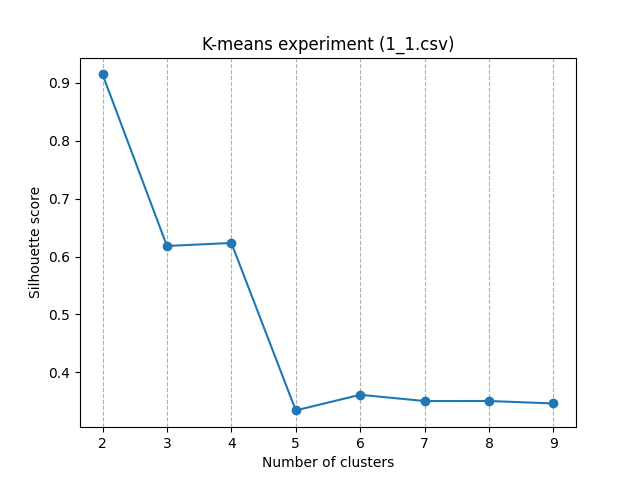
\includegraphics[width=\linewidth]{img/exp_1/kmeans/1_1_scores.png}
        \caption{Zbior 1\_1}
    \end{subfigure}
    \hfill
    \begin{subfigure}[b]{0.3\textwidth}
        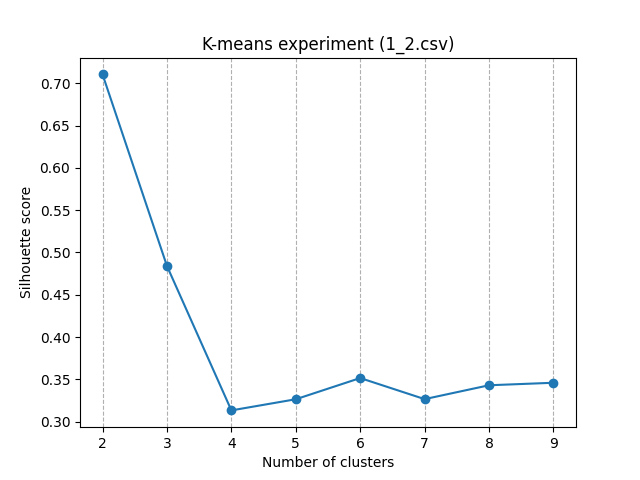
\includegraphics[width=\linewidth]{img/exp_1/kmeans/1_2_scores.png}
        \caption{Zbior 1\_2}
    \end{subfigure}
    \hfill
    \begin{subfigure}[b]{0.3\textwidth}
        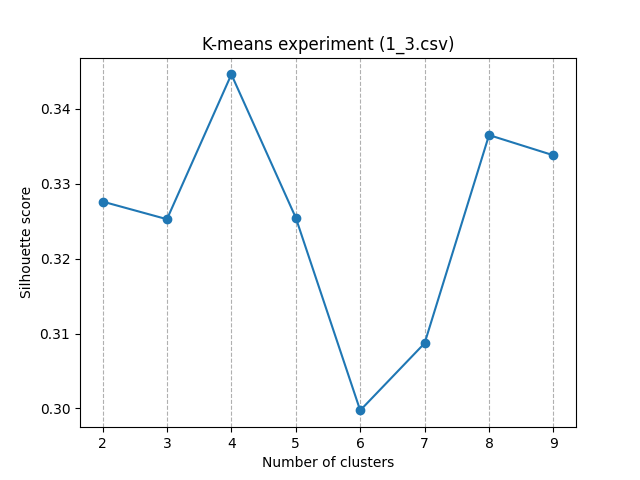
\includegraphics[width=\linewidth]{img/exp_1/kmeans/1_3_scores.png}
        \caption{Zbior 1\_3}
    \end{subfigure}
    \begin{subfigure}[b]{0.3\textwidth}
        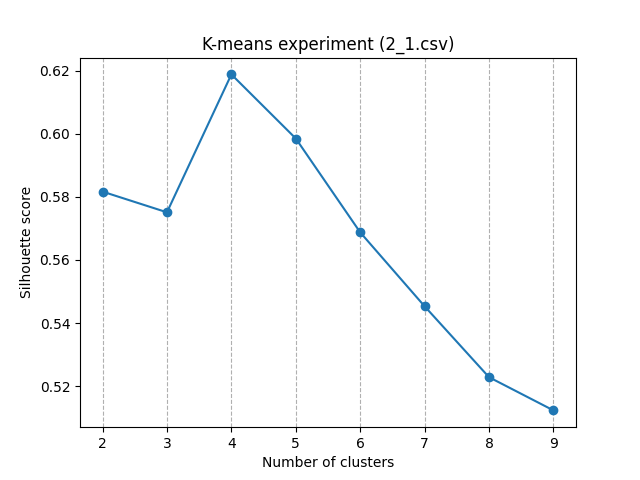
\includegraphics[width=\linewidth]{img/exp_1/kmeans/2_1_scores.png}
        \caption{Zbior 2\_1}
    \end{subfigure}
    \hfill
    \begin{subfigure}[b]{0.3\textwidth}
        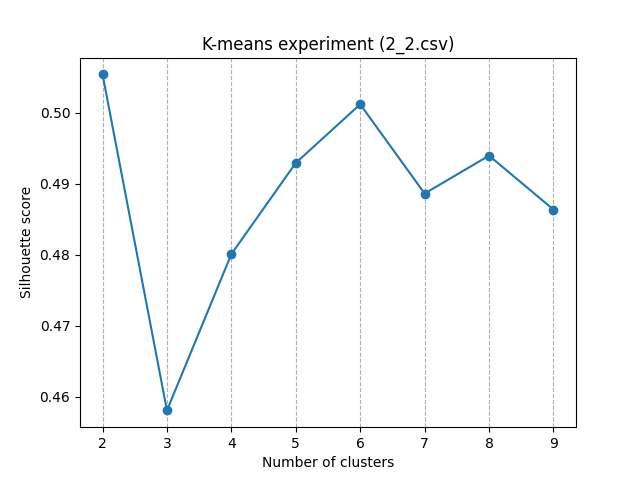
\includegraphics[width=\linewidth]{img/exp_1/kmeans/2_2_scores.png}
        \caption{Zbior 2\_2}
    \end{subfigure}
    \hfill
    \begin{subfigure}[b]{0.3\textwidth}
        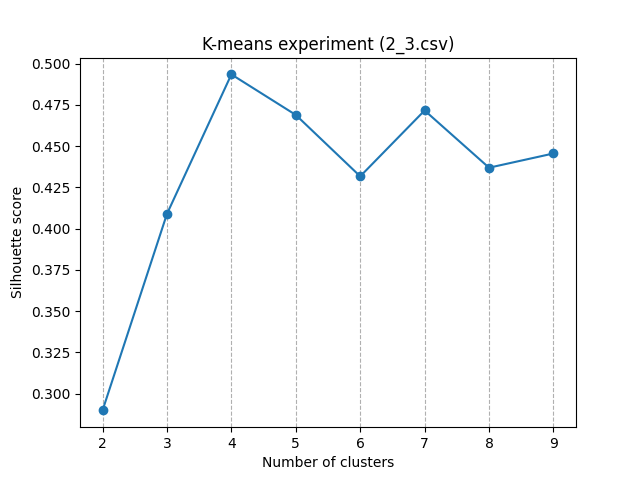
\includegraphics[width=\linewidth]{img/exp_1/kmeans/2_3_scores.png}
        \caption{Zbior 2\_3}
    \end{subfigure}
    \caption{\centering Zmiana wartości silhouette score dla wszystkich zbiorów w zależności od parametru n\_clusters w metodzie K-means}
\end{figure}

% Najlepszy i najgorszy przypadek dla wszystkich zbiorów
\begin{figure}[H]
    \centering
    \begin{subfigure}[b]{0.24\textwidth}
        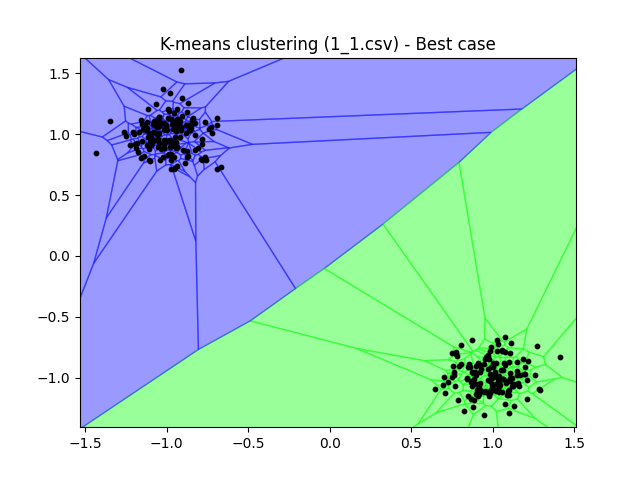
\includegraphics[width=\linewidth]{img/exp_1/kmeans/1_1_best.png}
        \caption{Najlepszy dla 1\_1}
    \end{subfigure}
    \hfill
    \begin{subfigure}[b]{0.24\textwidth}
        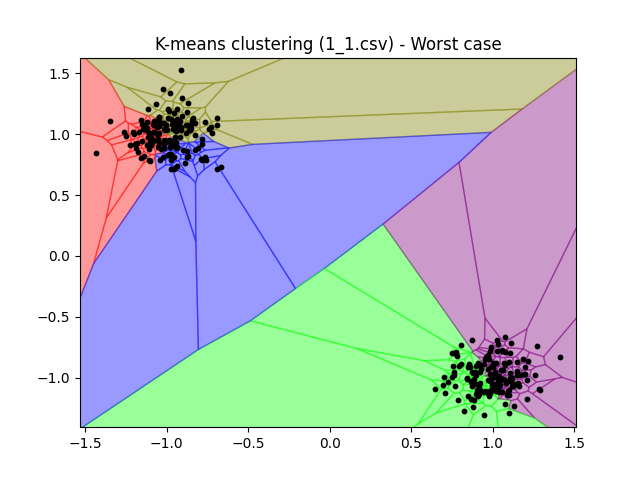
\includegraphics[width=\linewidth]{img/exp_1/kmeans/1_1_worst.png}
        \caption{Najgorszy dla 1\_1}
    \end{subfigure}
    \hfill
    \begin{subfigure}[b]{0.24\textwidth}
        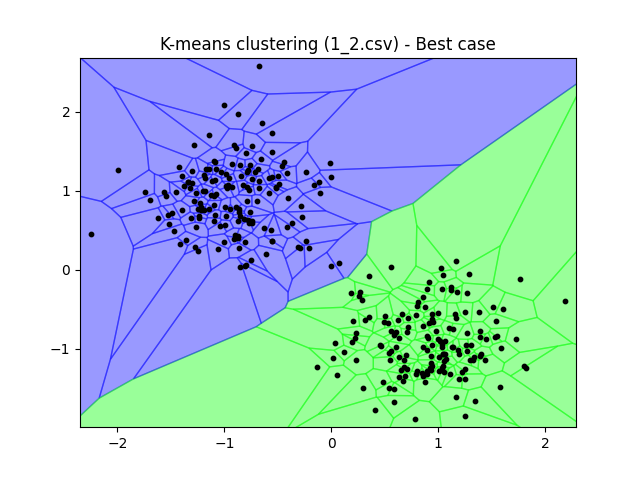
\includegraphics[width=\linewidth]{img/exp_1/kmeans/1_2_best.png}
        \caption{Najlepszy dla 1\_2}
    \end{subfigure}
    \hfill
    \begin{subfigure}[b]{0.24\textwidth}
        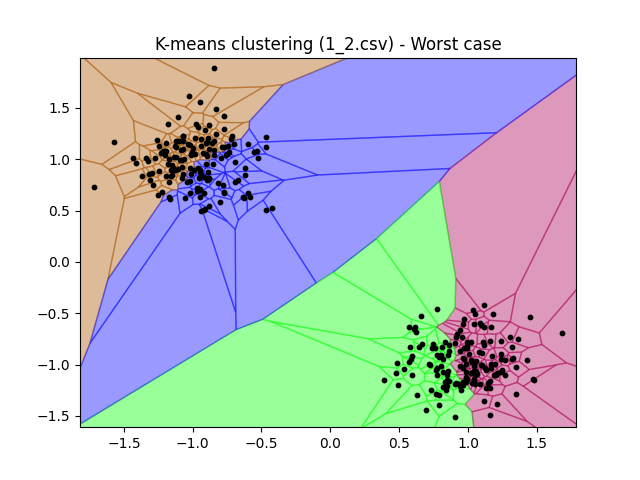
\includegraphics[width=\linewidth]{img/exp_1/kmeans/1_2_worst.png}
        \caption{Najgorszy dla 1\_2}
    \end{subfigure}
    \begin{subfigure}[b]{0.24\textwidth}
        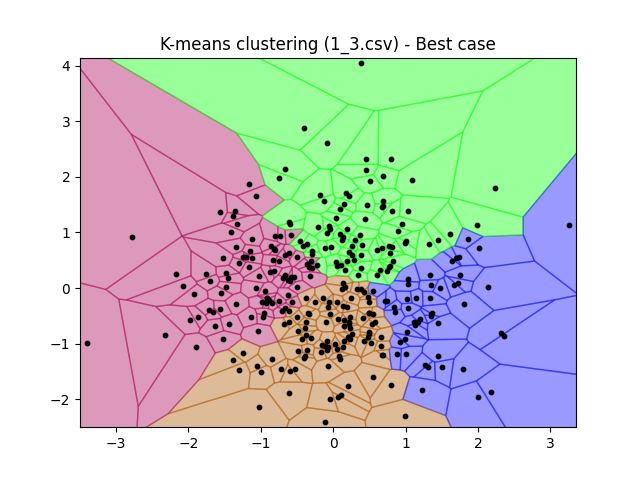
\includegraphics[width=\linewidth]{img/exp_1/kmeans/1_3_best.png}
        \caption{Najlepszy dla 1\_3}
    \end{subfigure}
    \hfill
    \begin{subfigure}[b]{0.24\textwidth}
        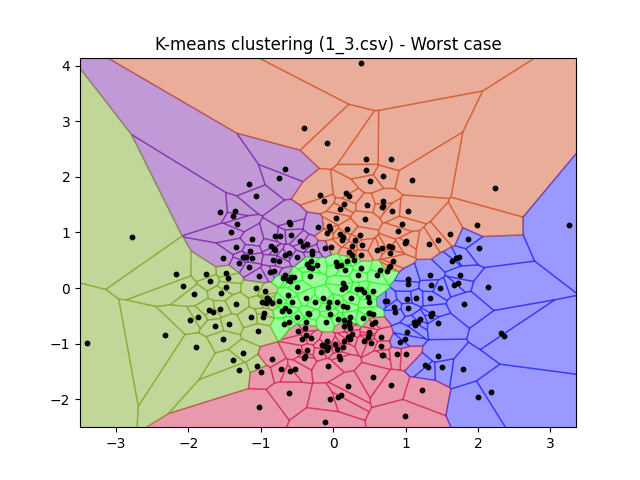
\includegraphics[width=\linewidth]{img/exp_1/kmeans/1_3_worst.png}
        \caption{Najgorszy dla 1\_3}
    \end{subfigure}
    \hfill
    \begin{subfigure}[b]{0.24\textwidth}
        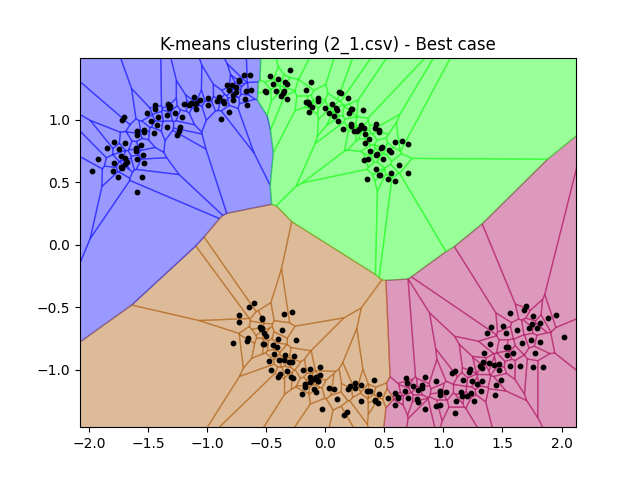
\includegraphics[width=\linewidth]{img/exp_1/kmeans/2_1_best.png}
        \caption{Najlepszy dla 2\_1}
    \end{subfigure}
    \hfill
    \begin{subfigure}[b]{0.24\textwidth}
        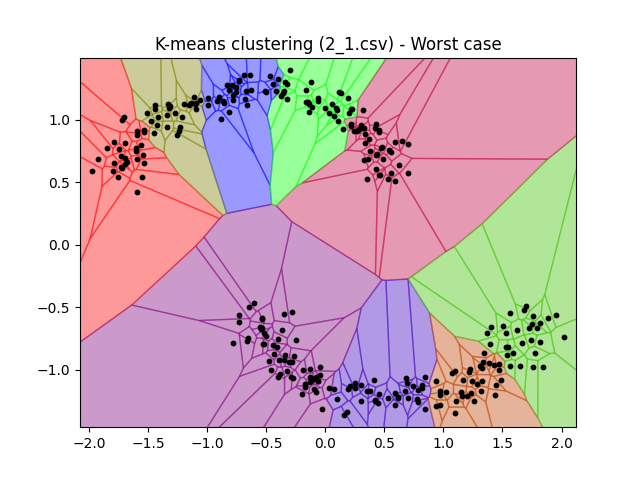
\includegraphics[width=\linewidth]{img/exp_1/kmeans/2_1_worst.png}
        \caption{Najgorszy dla 2\_1}
    \end{subfigure}
    \begin{subfigure}[b]{0.24\textwidth}
        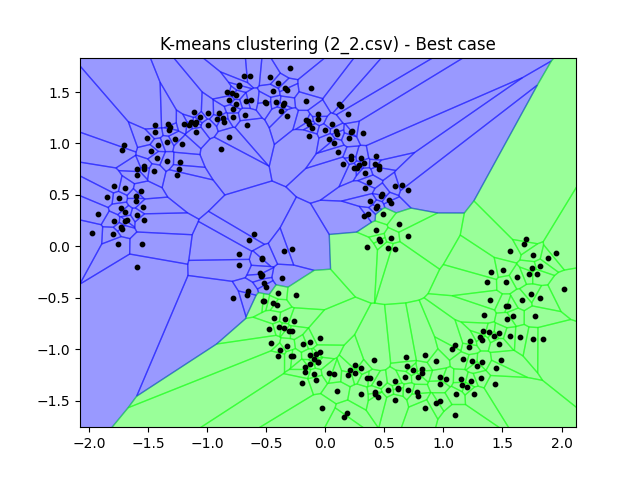
\includegraphics[width=\linewidth]{img/exp_1/kmeans/2_2_best.png}
        \caption{Najlepszy dla 2\_2}
    \end{subfigure}
    \hfill
    \begin{subfigure}[b]{0.24\textwidth}
        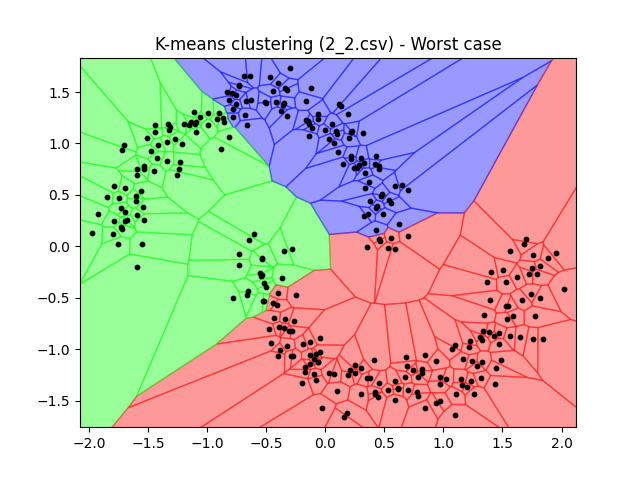
\includegraphics[width=\linewidth]{img/exp_1/kmeans/2_2_worst.png}
        \caption{Najgorszy dla 2\_2}
    \end{subfigure}
    \hfill
    \begin{subfigure}[b]{0.24\textwidth}
        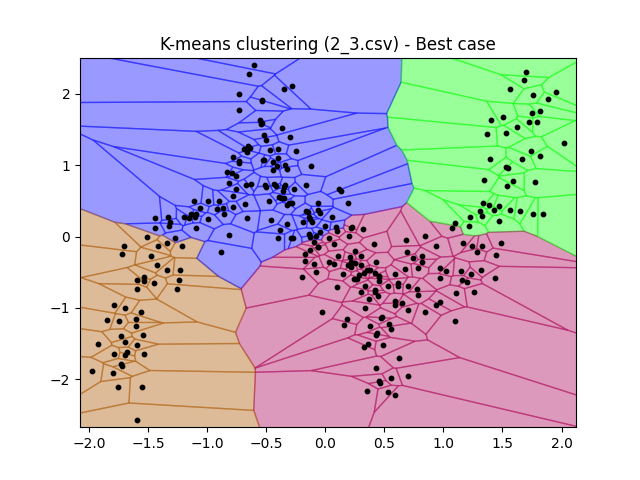
\includegraphics[width=\linewidth]{img/exp_1/kmeans/2_3_best.png}
        \caption{Najlepszy dla 2\_3}
    \end{subfigure}
    \hfill
    \begin{subfigure}[b]{0.24\textwidth}
        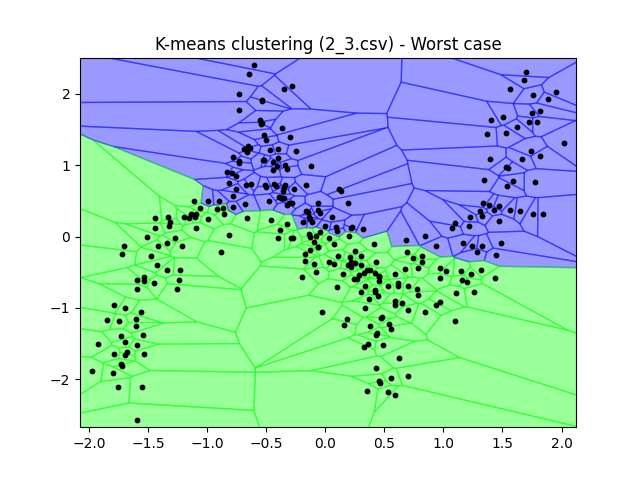
\includegraphics[width=\linewidth]{img/exp_1/kmeans/2_3_worst.png}
        \caption{Najgorszy dla 2\_3}
    \end{subfigure}
    \caption{\centering Wizualizacja klastrów dla wszystkich zbiorów na diagramie Voronoia dla najlepszego i najgorszego przypadku w metodzie K-means}
\end{figure}


\newpage
% DRUGA STRONA
\section{Eksperyment 1: Metoda DBSCAN}
% Wyniki dla Sztucznie Wygenerowanych Zbiorów Danych
\begin{figure}[H]
    \centering
    \begin{subfigure}[b]{0.3\textwidth}
        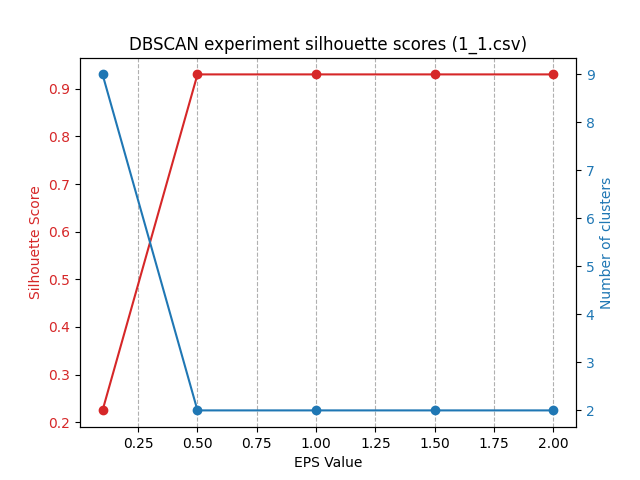
\includegraphics[width=\linewidth]{img/exp_1/dbscan/1_1_scores.png}
        \caption{Zbior 1\_1}
    \end{subfigure}
    \hfill
    \begin{subfigure}[b]{0.3\textwidth}
        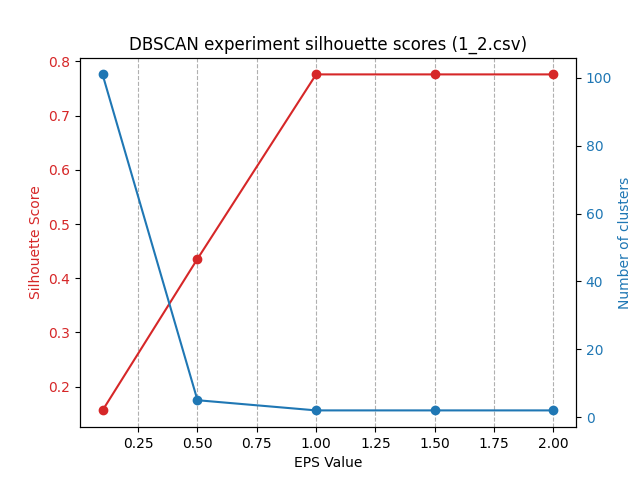
\includegraphics[width=\linewidth]{img/exp_1/dbscan/1_2_scores.png}
        \caption{Zbior 1\_2}
    \end{subfigure}
    \hfill
    \begin{subfigure}[b]{0.3\textwidth}
        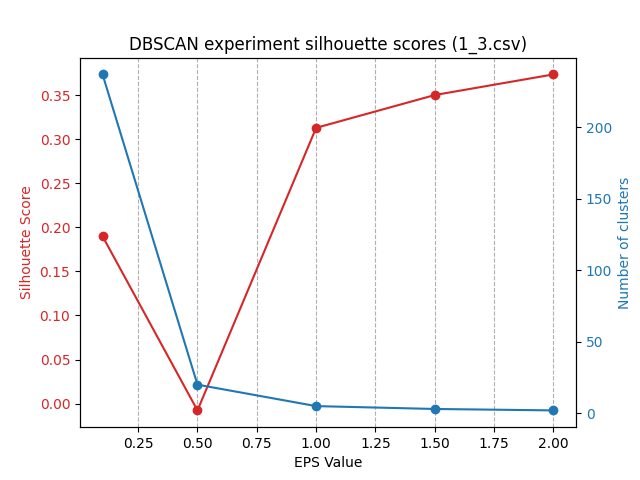
\includegraphics[width=\linewidth]{img/exp_1/dbscan/1_3_scores.png}
        \caption{Zbior 1\_3}
    \end{subfigure}
    \begin{subfigure}[b]{0.3\textwidth}
        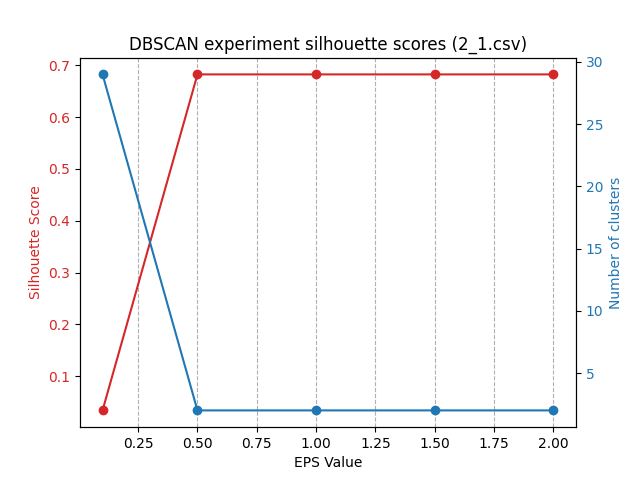
\includegraphics[width=\linewidth]{img/exp_1/dbscan/2_1_scores.png}
        \caption{Zbior 2\_1}
    \end{subfigure}
    \hfill
    \begin{subfigure}[b]{0.3\textwidth}
        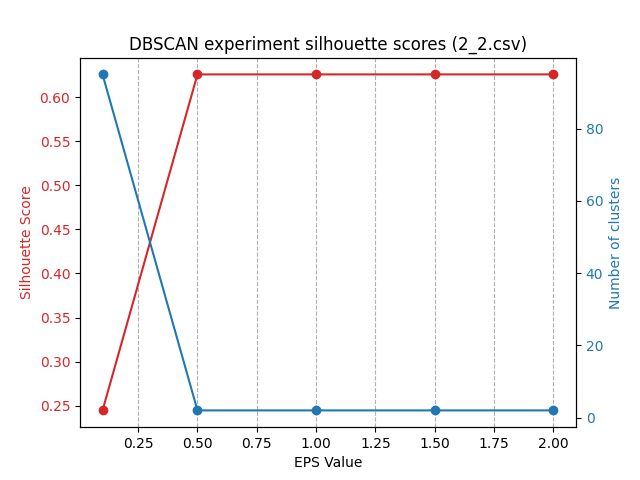
\includegraphics[width=\linewidth]{img/exp_1/dbscan/2_2_scores.png}
        \caption{Zbior 2\_2}
    \end{subfigure}
    \hfill
    \begin{subfigure}[b]{0.3\textwidth}
        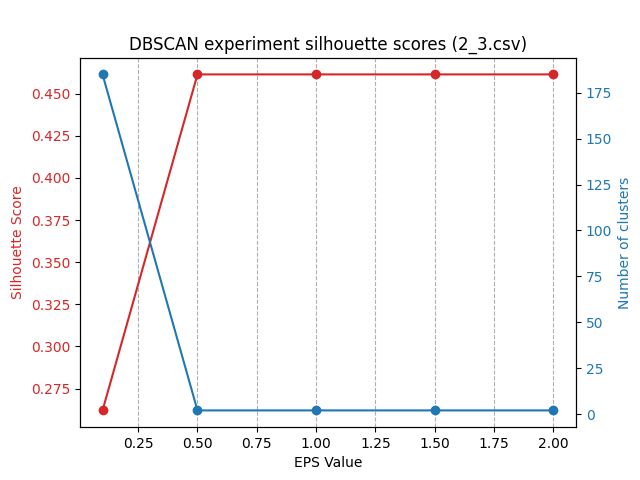
\includegraphics[width=\linewidth]{img/exp_1/dbscan/2_3_scores.png}
        \caption{Zbior 2\_3}
    \end{subfigure}
    \caption{\centering Zmiana wartości silhouette score oraz n\_clusters dla wszystkich zbiorów w zależności od zmieniającego się parametru eps w metodzie DBSCAN}
\end{figure}

% Najlepszy i najgorszy przypadek dla wszystkich zbiorów
\begin{figure}[H]
    \centering
    \begin{subfigure}[b]{0.24\textwidth}
        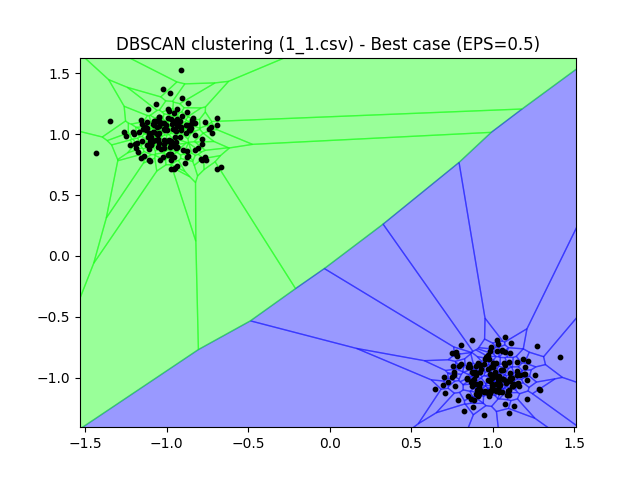
\includegraphics[width=\linewidth]{img/exp_1/dbscan/1_1_best.png}
        \caption{Najlepszy dla 1\_1}
    \end{subfigure}
    \hfill
    \begin{subfigure}[b]{0.24\textwidth}
        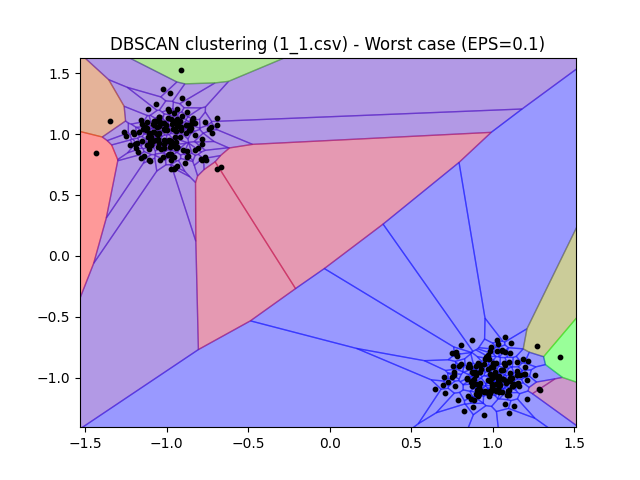
\includegraphics[width=\linewidth]{img/exp_1/dbscan/1_1_worst.png}
        \caption{Najgorszy dla 1\_1}
    \end{subfigure}
    \hfill
    \begin{subfigure}[b]{0.24\textwidth}
        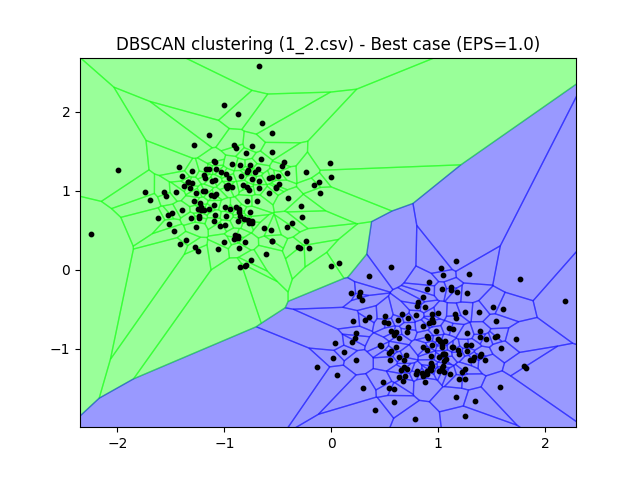
\includegraphics[width=\linewidth]{img/exp_1/dbscan/1_2_best.png}
        \caption{Najlepszy dla 1\_2}
    \end{subfigure}
    \hfill
    \begin{subfigure}[b]{0.24\textwidth}
        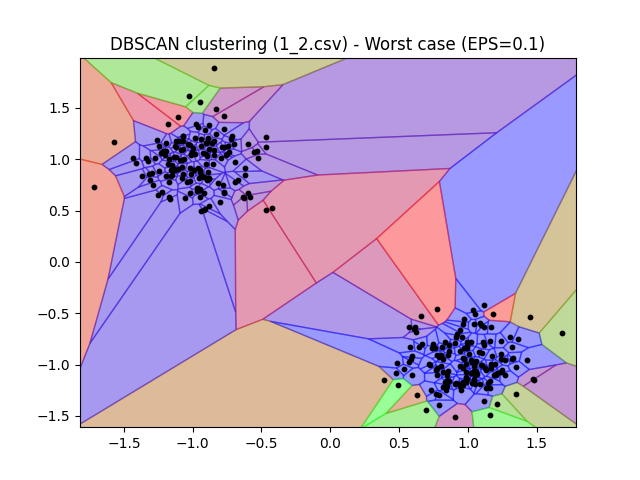
\includegraphics[width=\linewidth]{img/exp_1/dbscan/1_2_worst.png}
        \caption{Najgorszy dla 1\_2}
    \end{subfigure}
    \begin{subfigure}[b]{0.24\textwidth}
        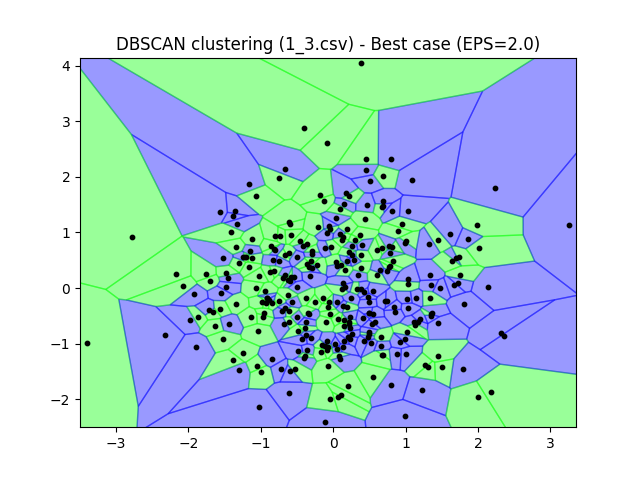
\includegraphics[width=\linewidth]{img/exp_1/dbscan/1_3_best.png}
        \caption{Najlepszy dla 1\_3}
    \end{subfigure}
    \hfill
    \begin{subfigure}[b]{0.24\textwidth}
        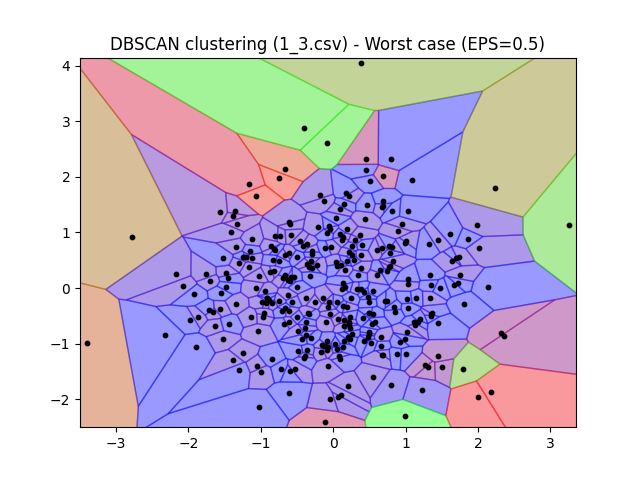
\includegraphics[width=\linewidth]{img/exp_1/dbscan/1_3_worst.png}
        \caption{Najgorszy dla 1\_3}
    \end{subfigure}
    \hfill
    \begin{subfigure}[b]{0.24\textwidth}
        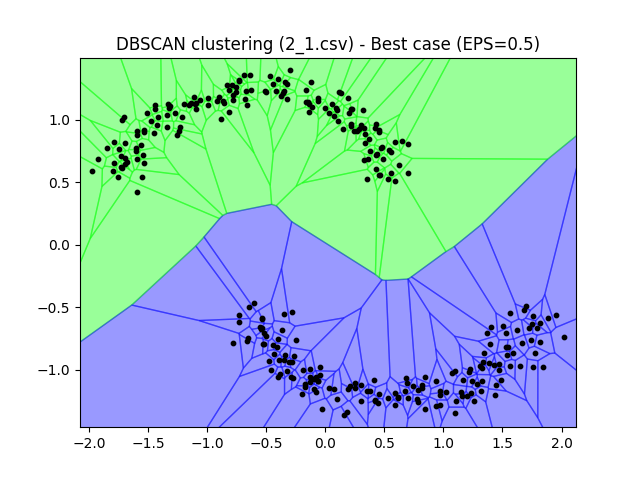
\includegraphics[width=\linewidth]{img/exp_1/dbscan/2_1_best.png}
        \caption{Najlepszy dla 2\_1}
    \end{subfigure}
    \hfill
    \begin{subfigure}[b]{0.24\textwidth}
        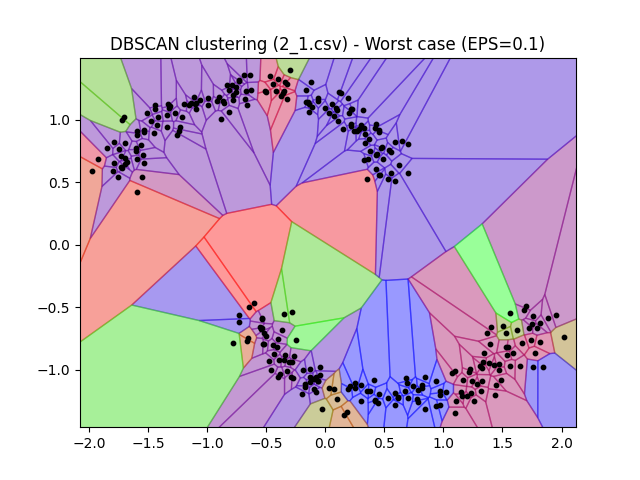
\includegraphics[width=\linewidth]{img/exp_1/dbscan/2_1_worst.png}
        \caption{Najgorszy dla 2\_1}
    \end{subfigure}
    \begin{subfigure}[b]{0.24\textwidth}
        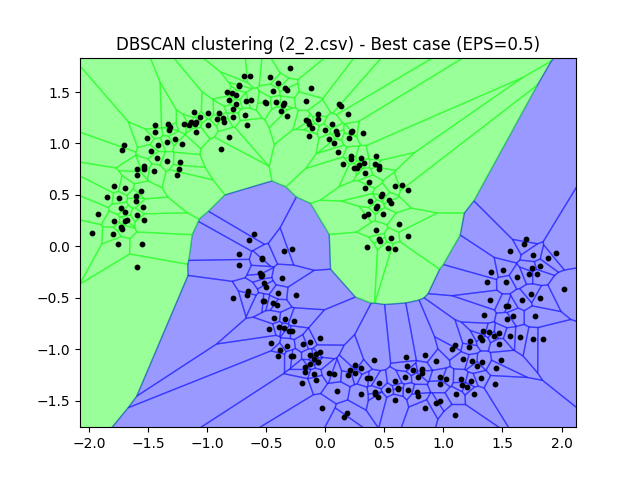
\includegraphics[width=\linewidth]{img/exp_1/dbscan/2_2_best.png}
        \caption{Najlepszy dla 2\_2}
    \end{subfigure}
    \hfill
    \begin{subfigure}[b]{0.24\textwidth}
        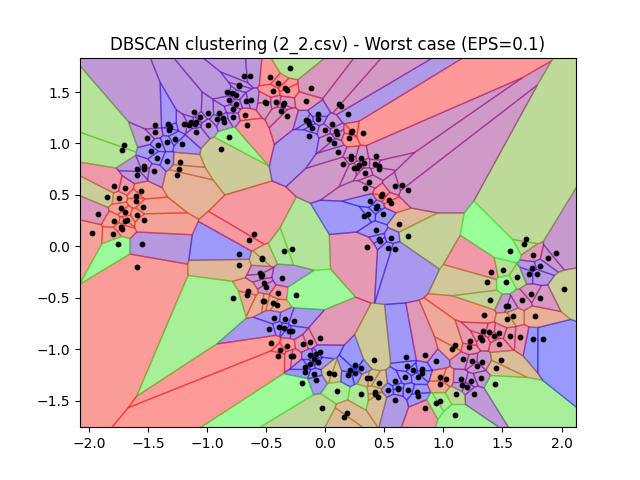
\includegraphics[width=\linewidth]{img/exp_1/dbscan/2_2_worst.png}
        \caption{Najgorszy dla 2\_2}
    \end{subfigure}
    \hfill
    \begin{subfigure}[b]{0.24\textwidth}
        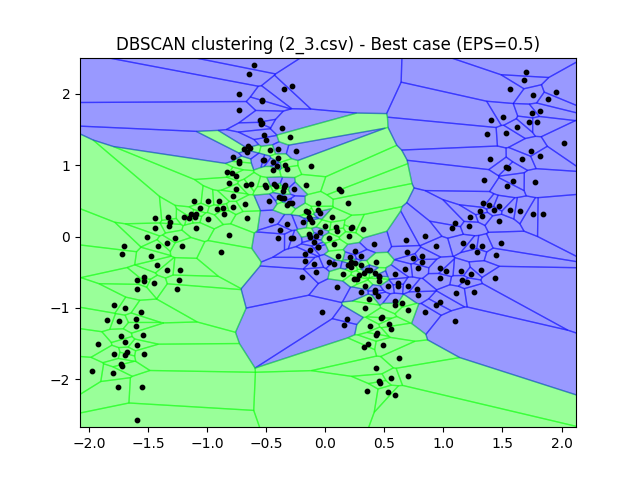
\includegraphics[width=\linewidth]{img/exp_1/dbscan/2_3_best.png}
        \caption{Najlepszy dla 2\_3}
    \end{subfigure}
    \hfill
    \begin{subfigure}[b]{0.24\textwidth}
        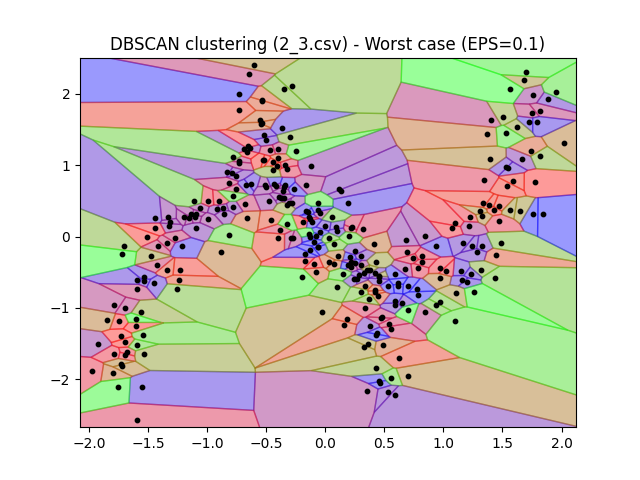
\includegraphics[width=\linewidth]{img/exp_1/dbscan/2_3_worst.png}
        \caption{Najgorszy dla 2\_3}
    \end{subfigure}
    \caption{\centering Wizualizacja klastrów dla wszystkich zbiorów na diagramie Voronoia dla najlepszego i najgorszego przypadku w metodzie DBSCAN}
\end{figure}

% TRZECIA STRONA
\section{Eksperyment 2: Metoda K-Means z etykietami}

% Wyniki drugiego eksperymentu dla sześciu sztucznie wygenerowanych zbiorów danych i metody K-Means. 
% Dla każdego zbioru należy pokazać wykres obrazujący zmianę wartości miar adjusted rand score, homogeneity score,  completeness score oraz V-measure score przy zmieniającym się parametrze n-clusters oraz wizualizację klastrów (diagram Woronoja z pokazanymi prawdziwymi etykietami obiektów) dla najlepszego i najgorszego przypadku (wskazując, który to był przypadek i dlaczego). 

\begin{figure}[H]
    \centering
    \begin{subfigure}[b]{0.3\textwidth}
        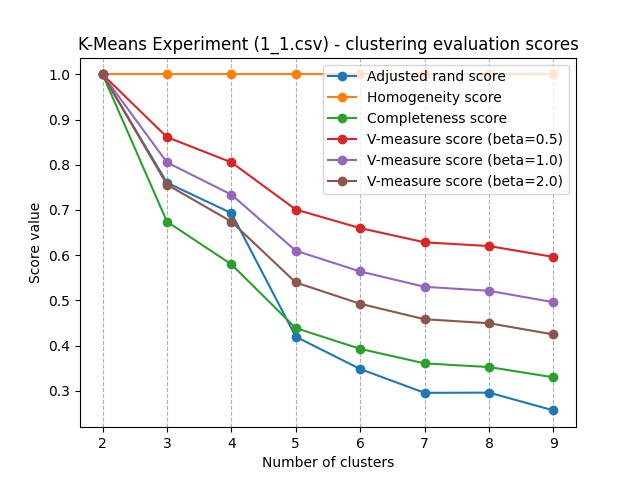
\includegraphics[width=\linewidth]{img/exp_2/kmeans/1_1_scores.png}
        \caption{Zbior 1\_1}
    \end{subfigure}
    \hfill
    \begin{subfigure}[b]{0.3\textwidth}
        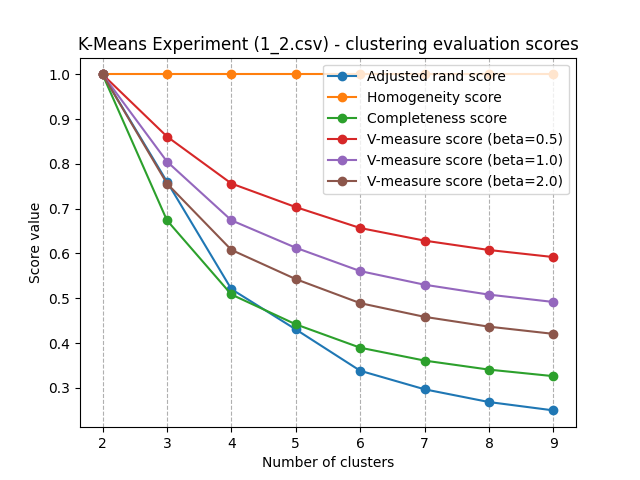
\includegraphics[width=\linewidth]{img/exp_2/kmeans/1_2_scores.png}
        \caption{Zbior 1\_2}
    \end{subfigure}
    \hfill
    \begin{subfigure}[b]{0.3\textwidth}
        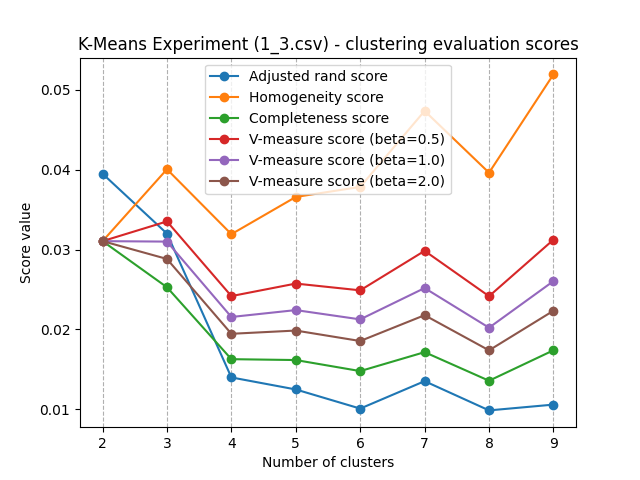
\includegraphics[width=\linewidth]{img/exp_2/kmeans/1_3_scores.png}
        \caption{Zbior 1\_3}
    \end{subfigure}
    \begin{subfigure}[b]{0.3\textwidth}
        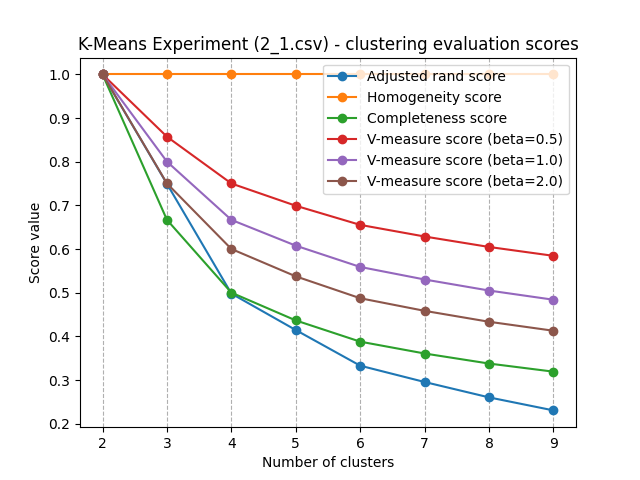
\includegraphics[width=\linewidth]{img/exp_2/kmeans/2_1_scores.png}
        \caption{Zbior 2\_1}
    \end{subfigure}
    \hfill
    \begin{subfigure}[b]{0.3\textwidth}
        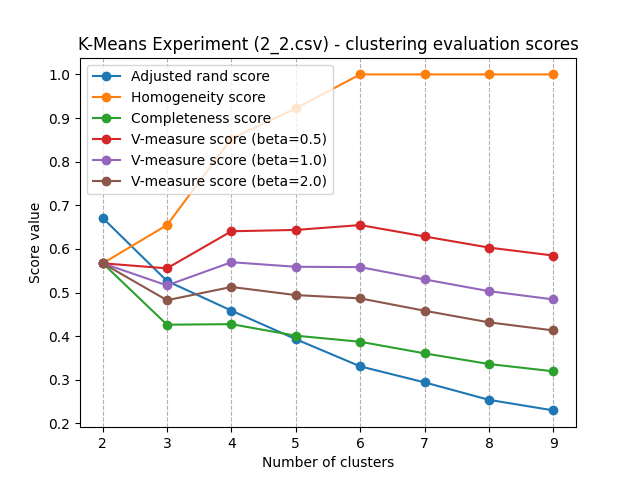
\includegraphics[width=\linewidth]{img/exp_2/kmeans/2_2_scores.png}
        \caption{Zbior 2\_2}
    \end{subfigure}
    \hfill
    \begin{subfigure}[b]{0.3\textwidth}
        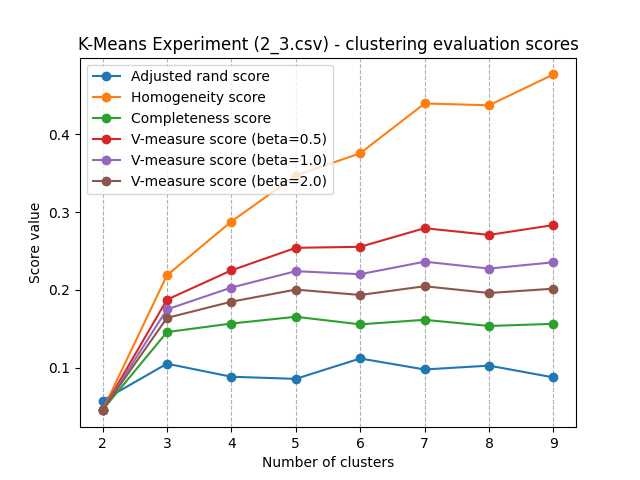
\includegraphics[width=\linewidth]{img/exp_2/kmeans/2_3_scores.png}
        \caption{Zbior 2\_3}
    \end{subfigure}
    \caption{\centering Zmiana wartości miar jakosći dla wszystkich zbiorów w zależności od liczby klastrów w metodzie K-means}
\end{figure}

\begin{figure}[H]
    \centering
    \begin{subfigure}[b]{0.24\textwidth}
        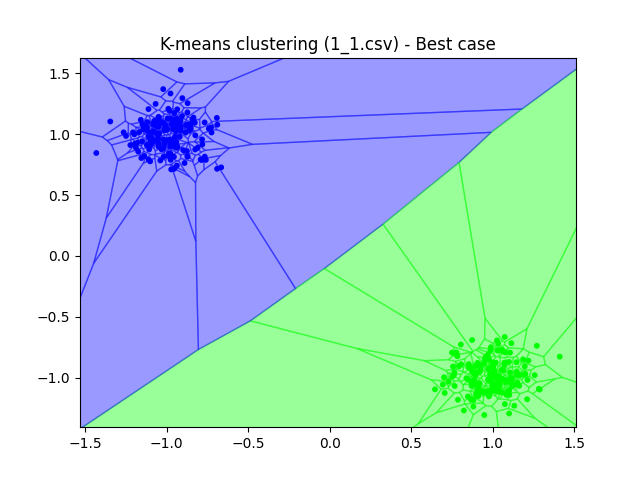
\includegraphics[width=\linewidth]{img/exp_2/kmeans/1_1_best.png}
        \caption{Najlepszy dla 1\_1}
    \end{subfigure}
    \hfill
    \begin{subfigure}[b]{0.24\textwidth}
        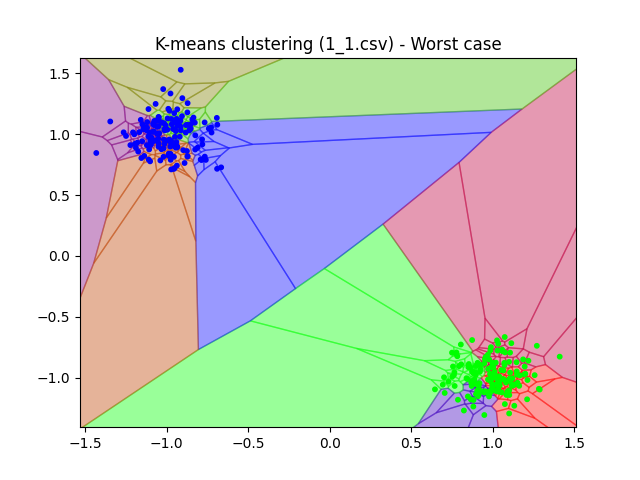
\includegraphics[width=\linewidth]{img/exp_2/kmeans/1_1_worst.png}
        \caption{Najgorszy dla 1\_1}
    \end{subfigure}
    \hfill
    \begin{subfigure}[b]{0.24\textwidth}
        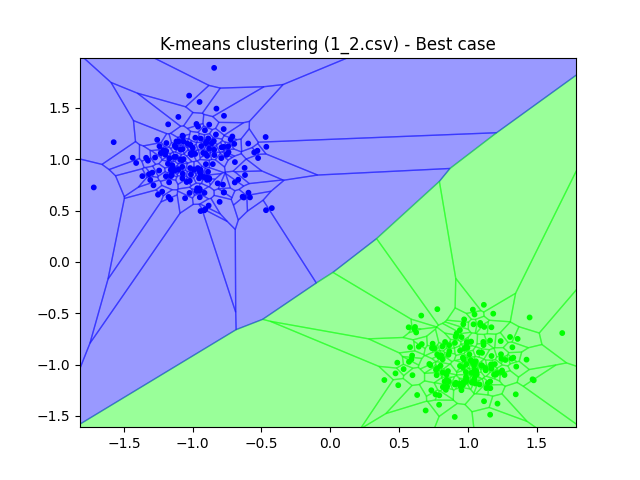
\includegraphics[width=\linewidth]{img/exp_2/kmeans/1_2_best.png}
        \caption{Najlepszy dla 1\_2}
    \end{subfigure}
    \hfill
    \begin{subfigure}[b]{0.24\textwidth}
        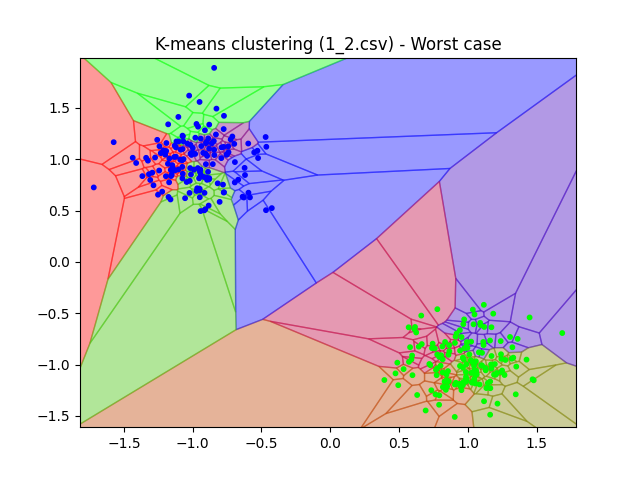
\includegraphics[width=\linewidth]{img/exp_2/kmeans/1_2_worst.png}
        \caption{Najgorszy dla 1\_2}
    \end{subfigure}
    \begin{subfigure}[b]{0.24\textwidth}
        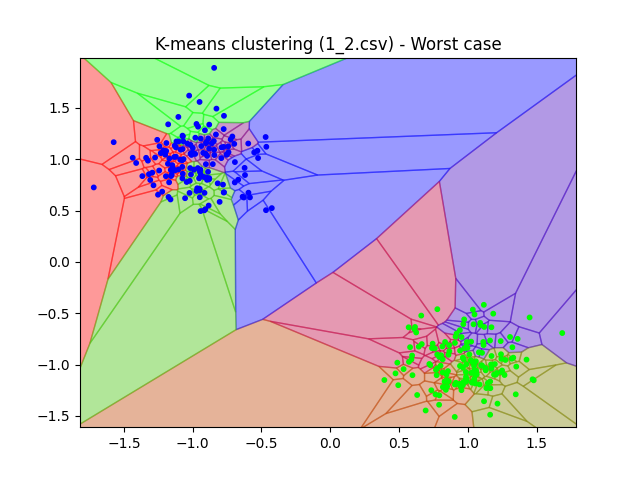
\includegraphics[width=\linewidth]{img/exp_2/kmeans/1_2_worst.png}
        \caption{Najlepszy dla 1\_3}
    \end{subfigure}
    \hfill
    \begin{subfigure}[b]{0.24\textwidth}
        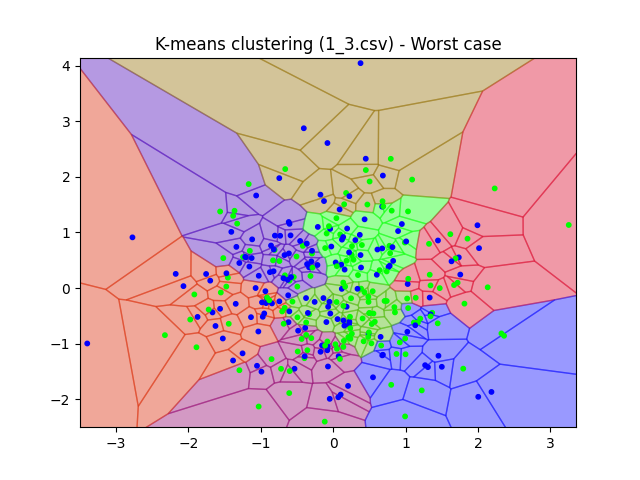
\includegraphics[width=\linewidth]{img/exp_2/kmeans/1_3_worst.png}
        \caption{Najgorszy dla 1\_3}
    \end{subfigure}
    \hfill
    \begin{subfigure}[b]{0.24\textwidth}
        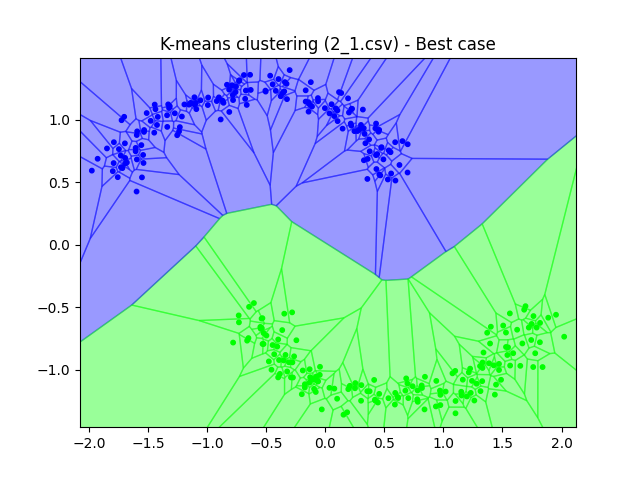
\includegraphics[width=\linewidth]{img/exp_2/kmeans/2_1_best.png}
        \caption{Najlepszy dla 2\_1}
    \end{subfigure}
    \hfill
    \begin{subfigure}[b]{0.24\textwidth}
        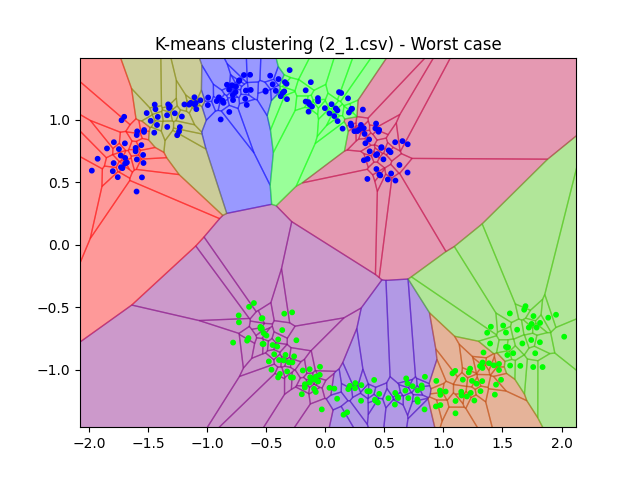
\includegraphics[width=\linewidth]{img/exp_2/kmeans/2_1_worst.png}
        \caption{Najgorszy dla 2\_1}
    \end{subfigure}
    \begin{subfigure}[b]{0.24\textwidth}
        \includegraphics[width=\linewidth]{img/exp_2/kmeans/2_2_best.png}
        \caption{Najlepszy dla 2\_2}
    \end{subfigure}
    \hfill
    \begin{subfigure}[b]{0.24\textwidth}
        \includegraphics[width=\linewidth]{img/exp_2/kmeans/2_2_worst.png}
        \caption{Najgorszy dla 2\_2}
    \end{subfigure}
    \hfill
    \begin{subfigure}[b]{0.24\textwidth}
        \includegraphics[width=\linewidth]{img/exp_2/kmeans/2_3_best.png}
        \caption{Najlepszy dla 2\_3}
    \end{subfigure}
    \hfill
    \begin{subfigure}[b]{0.24\textwidth}
        \includegraphics[width=\linewidth]{img/exp_2/kmeans/2_3_worst.png}
        \caption{Najgorszy dla 2\_3}
    \end{subfigure}
    \caption{\centering Wizualizacja klastrów wraz z prawdziwymi etykietami dla wszystkich zbiorów dla najlepszego i najgorszego przypadku w metodzie K-means}
\end{figure}

\newpage
% CZWARTA STRONA
\section{Eksperyment 2: Metoda DBSCAN z etykietami}

\begin{figure}[H]
    \centering
    \begin{subfigure}[b]{0.3\textwidth}
        \includegraphics[width=\linewidth]{img/exp_2/dbscan/1_1_scores.png}
        \caption{Zbior 1\_1}
    \end{subfigure}
    \hfill
    \begin{subfigure}[b]{0.3\textwidth}
        \includegraphics[width=\linewidth]{img/exp_2/dbscan/1_2_scores.png}
        \caption{Zbior 1\_2}
    \end{subfigure}
    \hfill
    \begin{subfigure}[b]{0.3\textwidth}
        \includegraphics[width=\linewidth]{img/exp_2/dbscan/1_3_scores.png}
        \caption{Zbior 1\_3}
    \end{subfigure}
    \begin{subfigure}[b]{0.3\textwidth}
        \includegraphics[width=\linewidth]{img/exp_2/dbscan/2_1_scores.png}
        \caption{Zbior 2\_1}
    \end{subfigure}
    \hfill
    \begin{subfigure}[b]{0.3\textwidth}
        \includegraphics[width=\linewidth]{img/exp_2/dbscan/2_2_scores.png}
        \caption{Zbior 2\_2}
    \end{subfigure}
    \hfill
    \begin{subfigure}[b]{0.3\textwidth}
        \includegraphics[width=\linewidth]{img/exp_2/dbscan/2_3_scores.png}
        \caption{Zbior 2\_3}
    \end{subfigure}
    \caption{\centering Zmiana wartości miar jakosći oraz liczba klastrów dla wszystkich zbiorów w zależności od wartosci eps w metodzie DBSCAN}
\end{figure}

\begin{figure}[H]
    \centering
    \begin{subfigure}[b]{0.24\textwidth}
        \includegraphics[width=\linewidth]{img/exp_2/dbscan/1_1_best.png}
        \caption{Najlepszy dla 1\_1}
    \end{subfigure}
    \hfill
    \begin{subfigure}[b]{0.24\textwidth}
        \includegraphics[width=\linewidth]{img/exp_2/dbscan/1_1_worst.png}
        \caption{Najgorszy dla 1\_1}
    \end{subfigure}
    \hfill
    \begin{subfigure}[b]{0.24\textwidth}
        \includegraphics[width=\linewidth]{img/exp_2/dbscan/1_2_best.png}
        \caption{Najlepszy dla 1\_2}
    \end{subfigure}
    \hfill
    \begin{subfigure}[b]{0.24\textwidth}
        \includegraphics[width=\linewidth]{img/exp_2/dbscan/1_2_worst.png}
        \caption{Najgorszy dla 1\_2}
    \end{subfigure}
    \begin{subfigure}[b]{0.24\textwidth}
        \includegraphics[width=\linewidth]{img/exp_2/dbscan/1_2_worst.png}
        \caption{Najlepszy dla 1\_3}
    \end{subfigure}
    \hfill
    \begin{subfigure}[b]{0.24\textwidth}
        \includegraphics[width=\linewidth]{img/exp_2/dbscan/1_3_worst.png}
        \caption{Najgorszy dla 1\_3}
    \end{subfigure}
    \hfill
    \begin{subfigure}[b]{0.24\textwidth}
        \includegraphics[width=\linewidth]{img/exp_2/dbscan/2_1_best.png}
        \caption{Najlepszy dla 2\_1}
    \end{subfigure}
    \hfill
    \begin{subfigure}[b]{0.24\textwidth}
        \includegraphics[width=\linewidth]{img/exp_2/dbscan/2_1_worst.png}
        \caption{Najgorszy dla 2\_1}
    \end{subfigure}
    \begin{subfigure}[b]{0.24\textwidth}
        \includegraphics[width=\linewidth]{img/exp_2/dbscan/2_2_best.png}
        \caption{Najlepszy dla 2\_2}
    \end{subfigure}
    \hfill
    \begin{subfigure}[b]{0.24\textwidth}
        \includegraphics[width=\linewidth]{img/exp_2/dbscan/2_2_worst.png}
        \caption{Najgorszy dla 2\_2}
    \end{subfigure}
    \hfill
    \begin{subfigure}[b]{0.24\textwidth}
        \includegraphics[width=\linewidth]{img/exp_2/dbscan/2_3_best.png}
        \caption{Najlepszy dla 2\_3}
    \end{subfigure}
    \hfill
    \begin{subfigure}[b]{0.24\textwidth}
        \includegraphics[width=\linewidth]{img/exp_2/dbscan/2_3_worst.png}
        \caption{Najgorszy dla 2\_3}
    \end{subfigure}
    \caption{\centering Wizualizacja klastrów wraz z prawdziwymi etykietami dla wszystkich zbiorów dla najlepszego i najgorszego przypadku w metodzie DBSCAN}
\end{figure}

\newpage
% PIĄTA STRONA
\section{Wnioski}
Opis wniosków z eksperymentów przeprowadzonych na sześciu sztucznie wygenerowanych zbiorach. W przypadku pierwszego eksperymentu należy stwierdzić, jak, obserwując silhouette score, można dobrrać właściwe parametry metod klasteryzacji, aby klastry dobrze odkrywały strukturę danych. Dla eksperymentu drugiego należy wskazać jakie informację o separowalności klas można wycią obserwując wartości miar: adjusted rand score, homogeneity score,  completeness score oraz V-measure score. Wnioski powinny mieć charakter ogólny, pozwalający przenieść je na przypadek, w którym nie ma możliwości zwizualizowania danych. Każdy wniosek powinien być poparty odniesieniami do wyników przedstawionych na pierwszych czterech stronach raportu.

\subsection*{Eksperyment 1}



\subsection*{Eksperyment 2}

.

\subsection*{Analiza}

Analiza pozostałych, rzeczywistych zbiorów danych powinna uwzględniać wnioski z poprzednich eksperymentów. Można je również uzasadnić poprzez odwołanie do wartości miar uzyskanych na tych zbiorach.


\newpage
% SZÓSTA STRONA
\section{Analiza pozostałych zbiorów danych}
Opis analizy pozostałych, rzeczywistych zbiorów danych, w której to zastosowane zostaną wnioski z wcześniejszych eksperymentów. Wyniki tej analizy należy również uzasadnić poprzez odwołanie do wartości miar uzyskiwanych na tych zbiorach (warto wykorzystać tabele i/lub wykresy i się do nich odwołać). W przypadku zbioru Iris da się swoje wnioski podeprzeć wizualizacjami rzutów cech obiektów na dwuwymiarowe przestrzenie wybranych kombinacji dwóch z nich.

\subsection*{Wnioski}

Na podstawie przeprowadzonych eksperymentów możemy wnioskować o strukturze rzeczywistych zbiorów danych i skuteczności wybranych metod klasteryzacji.

\subsection*{Zbiór Iris}

\subsection*{Zbiór Wine}

\subsection*{Zbiór Breast Cancer Wisconsin}






\end{document}
